\documentclass[a4paper,12pt,hyperref,twoside]{ctexart}
\usepackage{amscd,amssymb,amsfonts,amsbsy,amsmath,verbatim} % 各种数学符号
%\usepackage{xeCJK}
%\usepackage{mathrsfs} %哥特体
%\usepackage{ntheorem}  % 定理环境
\usepackage{enumitem}  % 设置各条例间距
\usepackage{multicol}  % 多栏排版
\usepackage{color} % 字体和背景颜色
\usepackage{graphicx} %加载图片
\usepackage{subfigure}
\usepackage{paralist}
\usepackage{fancyhdr}
%\usepackage{picins} %文字环绕图片
%\usepackage{CJK}%支持中、日、韩文
%\usepackage{CJKulem} %加下划线的文本部分中可以断行
%\usepackage{CJKpunct} %调整中文标点后的空白
\usepackage{setspace} %设置行间距
\usepackage[left=3cm,right=2.5cm,top=3cm,bottom=2.5cm]{geometry} %页边距设定 上3cm 下2.5cm 左3cm 右2.5cm
%\usepackage{titlesec} %改变章节标题格式
\usepackage{times} %英文字体
\usepackage{xifthen} %使用\ifthenelse命令,必须要有这个包!
\usepackage{indentfirst} %首行缩进
\usepackage{makecell}    %表格宏包
\usepackage{enumitem}    %扩展列表
\usepackage{booktabs,array}
\usepackage{tikz}        %绘图
\usetikzlibrary{intersections} %tikz拓展
\usetikzlibrary{calc}          %tikz拓展
\usepackage{ifthen}      %分支程序
%\usepackage{bm}          %数学环境粗体 在xelatex下不可使用
\usepackage{multirow}    %多行表格
\usepackage{setspace}    %段落间距宏包
\usepackage{float}  %浮动表格图片
\usepackage{etex,yhmath} %数学符号
\usepackage{titletoc} %用于重定义目录格式
\usepackage{theorem}
\usepackage{cprotect}
%参考文献引用设定
\usepackage[backend=biber,style=gb7714-2015,gbalign=gb7714-2015,gbpub=false]{biblatex}
\addbibresource[location=local]{reference.bib} 
%\usepackage{gbt7714} %中文参考文献格式
%\bibliographystyle{gbt7714-numerical}
% 顺序编码制
\setmainfont{Times New Roman}
%\let\kaishu\relax%清除旧定义
%\newCJKfontfamily\kaishu{KaiTi}[AutoFakeBold] %使得楷书能够正常加粗
%\let\fangsong\relax%清除旧定义
%\newCJKfontfamily\fangsong{FangSong}[AutoFakeBold] %使得仿宋能够正常加粗
%\letti\relax%清除旧定义
%\newCJKfontfamilyti{SimSun}[AutoFakeBold] %使得宋体能够正常加粗
%%%%%临时新定义
\newcommand{\MakeBox}[3][s]
    {\makebox[#2\ccwd][#1]{\let \CJKglue \hfill #3}}
\newcommand{\MB}[3][c]
    {\makebox[#2\ccwd][#1]{#3}}
    %%%%%%%%%%%% 插图命令简化
\newcommand{\insertjpg}[2][\textwidth]
{\includegraphics[width=#1]{#2}}

\newcommand\setcolsep[1][2]   %微调列宽
    {\setlength\arraycolsep{#1pt}}

\newcommand{\dev}[2][]{{\,\textup{d}}^{#1}#2}   %%%用于输入dx!!
%%%%%%颜色
\def\white#1{\textcolor{white}{#1}}
\def\red#1{\textcolor{red}{#1}}
\def\blue#1{\textcolor{blue}{#1}}

%向量
\def\orarrow{\overrightarrow}

%%%%%%%%%%%%%%% 反斜 三点 idot
% \cdot \dots \ddots \dots \ldots
\def\idots{{\mathinner{\mkern2mu\raise1pt\hbox{.}\mkern2mu
        \raise4pt\hbox{.}\mkern2mu\raise7pt\hbox{.}\mkern1mu}} }
%\setCJKmainfont[BoldFont={SimHei}]{SimSun}
%%%% 字体
%\newcommand{}{\CJKfamily{simsun}} %宋体

%\newcommand{\kai}{\CJKfamily{kai}} %楷体
%\newcommand{\heiti}{\CJKfamily{SimHei}} %黑体
%\newcommand{\fangsong}{\CJKfamily{fs}} %仿宋
\setlength{\parindent}{2em} %设置段首缩进量
%%%%%% 页面设置
\pagestyle{fancy}%使用fancy做页面格式设置
\fancyhf{} %清除所有页眉页脚
\cfoot{\thepage}%页脚居中页码
\renewcommand{\headrulewidth}{0pt} %取消页眉中的装饰分割线
\renewcommand{\footrulewidth}{0pt} %取消页脚中的装饰分割线
%\renewcommand{\baselinestretch}{5.5}
\zihao{-4}
\linespread{1.5}  % 1.5倍行间距
%\baselineskip=23pt
\parskip=0pt      %段间距与行间距相等
\widowpenalty=0 
\clubpenalty=0000
%完全不控制孤行 这个值越大,控制力度越强 默认为150
%其中widowpentalty是出现尾行分页所产生的惩罚值,clubpenalty是出现首行分页的惩罚值。
\allowdisplaybreaks  %允许多行公式换页
%%%% 重定义标准大小
\makeatletter
\renewcommand{\normalsize}{%
   \@setfontsize\normalsize\@xpt\@xiipt
   \abovedisplayskip 4\p@ \@plus2\p@ \@minus5\p@
   \abovedisplayshortskip \z@ \@plus3\p@
   \belowdisplayshortskip 4\p@ \@plus3\p@ \@minus3\p@
   \belowdisplayskip \abovedisplayskip
   \let\@listi\@listI}
 %%%%先把\bf改为\textbf
   %一级标题格式
 \renewcommand\section{%
 \@startsection{section}{2}{0mm}{10pt}{8pt}%
 {\zihao{3}\textbf}%
}
% 二级标题格式
\renewcommand\subsection{%
 \@startsection{subsection}{2}{0mm}{0.1\baselineskip}{5pt}%
 {\zihao{-3}\textbf}%
}
% 三级标题格式
\renewcommand\subsubsection{%
 \@startsection{subsubsection}{0}{0mm}{0\baselineskip}{1pt}%
 {\zihao{4}\textbf\!\!}%
}
% 四级标题格式
\renewcommand\paragraph{%
 \@startsection{paragraph}{1}{0mm}{0.5\baselineskip}{0.5\baselineskip}%
 {\zihao{-4}\textbf}%
}
\makeatother

%%%%%%%% 目录格式
\setcounter{tocdepth}{2}
\renewcommand{\contentsname}{\centerline{\heiti\zihao{-2}目\quad 录}}

    % 一级标题
\titlecontents{section}
              [0em]
              {\zihao{-4} \addvspace{2bp minus 1bp}}
              {\contentslabel{0em}\quad}
              {}
              {\dotfill\textrm{\contentspage[\thecontentspage]}}
    % 二级标题
\titlecontents{subsection}
              [3.0em]
              {\zihao{-4}  \addvspace{1bp minus 1bp}}
              {\contentslabel{2.0em}}
              {}
              {\dotfill\textrm{\contentspage[\thecontentspage]}}

    % 三级标题, 此版本不显示此层次标题
    \titlecontents{subsubsection}
              [3.0em]
              {\zihao{-4} \addvspace{1bp minus 1bp}}
              {\contentslabel{2.0em}}
              {}
              {\dotfill\textrm{\contentspage[\thecontentspage]}}

%各种环境的距离设置
\renewcommand{\figurename}{\zihao{-5}图}
\renewcommand\tablename{\zihao{-5}表}

%页边距
\oddsidemargin=0pt
\evensidemargin=0pt
\setlength{\parindent}{2em} %设置段首缩进量
%%%%%%%%% 定理环境
\def\kg{\mbox{} \qquad } %手动空格指令
\newtheorem{thm}{\phantom{参数}定理}[section] %定理编号带有节前缀
\newtheorem{cor}[thm]{\phantom{参数}推论}
\newtheorem{prop}[thm]{\phantom{参数}命题}
\newtheorem{propt}[thm]{\phantom{参数}性质}
\newtheorem{lemma}[thm]{\phantom{参数}引理}
\newtheorem{definition}[thm]{\phantom{参数}定义}
\newtheorem{eg}[thm]{\phantom{参数}例}
\newtheorem{ques}[thm]{\phantom{参数}问题}
\newtheorem{exa}{\phantom{参数}例}[section]
\newtheorem{conj}[thm]{\phantom{参数}猜想}
\newtheorem{rema}[thm]{\phantom{参数}注}
\numberwithin{equation}{section}

%%%%%% 证明环境
\newenvironment{proof}[1][\indent 证明]
    {\textbf {#1}:~}
    {\hfill $\Box$}
\setlength{\theorempreskipamount}{0pt}%调整定理环境与上文的距离
\setlength{\theorempostskipamount}{0pt}%调整定理环境与下文的距离
%%%%%%%% 列表环境
\renewcommand{\labelitemi}{$\bullet$}
\def\myback{\vspace*{-25pt}}
\def\myhalfback{\vspace*{-12.5pt}}
%%%%%%%%%%%% 定理环境结束

\begin{document}
%%%%%%%%%% 以下内容为自动生成, 不需要修改.
\pagestyle{empty}\def\lnlen{8}
\vspace*{5mm} {\zihao{4}\fangsong
\MakeBox3{\bfseries 分类号}\underline{\MakeBox[c]\lnlen{}}\MakeBox{3}{}
\MakeBox{6}{\bfseries 论文选题类型}\underline{\MakeBox{6}{}}
\bigskip

\MakeBox{3}{\bfseries U\,\,D\,\,C}\underline{\MakeBox\lnlen{ }}\MakeBox{3}{}
\MakeBox2{\bfseries 编号}\underline{\MakeBox{10}{}}
\vspace*{15mm}

\begin{center}
%\zihao{2}

\insertjpg[.43\textwidth]{school.jpg}

\vspace*{18mm}
{\heiti \zihao{-1} \quad 本科毕业论文(设计)}
\end{center}}

\vspace*{15mm}\zihao{-3}
\newlength\titlelength
\newlength\testlength
\newlength\majorlen

%%%%%%%%%% majorlen记录个人信息中最长一行的长度
\settowidth\majorlen{数\!学\!与\!应\!用\!数\!学(师\!范)}%专业
\settowidth\testlength{数学与统计学学院}%学校
\ifthenelse{\testlength>\majorlen}
    {\setlength\majorlen{\testlength}}{}
\settowidth\testlength{张三丰 教授 \quad 三丰 教授}%老师
\ifthenelse{\testlength>\majorlen}
    {\setlength\majorlen{\testlength}}{}

%%%%%%%%% 论文题目
\settowidth\titlelength{\,浅谈我们的我们的大学的大大大学我们的大学的大大大大\,}
\setlength\testlength{16\ccwd+.5\ccwd}%单行题目长度
%\def\unlen{2.2*\mytitlenum/16} %16个汉字, 2.2

\begin{center}
\begin{tikzpicture}[scale=2]
    \pgfmathsetmacro{\h}{.45}
    \pgfmathsetmacro{\v}{1}
    \ifthenelse{\titlelength>\testlength}
        {%
        \draw(\h+1.4,\v/5)node[below]
            {\parbox[t][2cm][s]{.5\ccwd+16\ccwd}{%
            \begin{spacing}{1.95}
            \centering \zihao{-2}\textbf{浅谈我们的我们的大学的大大大学我们的大学的大大大大}
            \end{spacing}
            }};
            \foreach \i in {0,1}
                \foreach \j in {1,-1}
                    \draw[thick](\h*1.5+1.2,-\v/5-\i*\v*.75) --++({\j*\testlength/3.8},0);

            }
        {\draw(\h+1.4,\v/5-\v*.45)node[below]{\textbf{ti 浅谈我们的我们的大学的大大大学我们的大学的大大大大}};
        \foreach \j in {1,-1}
        \draw[thick](\h*1.5+1.2,-\v/5-\v*.42) --++({\j*\testlength/3.8},0);
        }
    \foreach \i/\text/\tex in {%
            1/学院/数学与统计学学院,
            2/专业/数\!学\!与\!应\!用\!数\!学(师\!范),
            3/年级/2017级,
            4/学生姓名/作者,
            5/学号/2015123456,
            6/指导教师/张三丰 教授 \quad 三丰 教授
            }
        {%
        \draw(-.3,{-1.8-\i*\v/2})node[right]{%
            \MakeBox4{\zihao{-3}\textbf{\text}}};
        \draw[thick](1.2,{-1.95-\i*\v/2})-- node[yshift=3mm]{\zihao{-3} \textbf{\tex}}++(\majorlen/1.92,0);}
    \draw(1.7,-6*\v)node{%
        \heiti\makebox[4\ccwd][c]{%
            二〇二一}\,\,年\,\,四\,\,月}; 
    \end{tikzpicture}
\end{center}
%%%%%%% 封面结束

%下面内容为版权页
\newpage
\thispagestyle{empty}
\newgeometry{left=2.85cm,right=2.45cm,top=3cm,bottom=2.5cm}
\zihao{4}
\centerline{\bfseries{\kaishu\zihao{-2}华中师范大学}}\vspace*{15pt}

\centerline{\bfseries \kaishu\zihao{-2}学位论文原创性声明}%
\vspace*{40pt}

\begin{spacing}{1.65}
\zihao{-4}

本人郑重声明:所呈交的学位论文是本人在导师指导下独立进行研究工作所取得的研究成果。除了文中特别加以标注引用的内容外,本论文不包含任何其他个人或集体已经发表或撰写的成果作品。本人完全意识到本声明的法律后果由本人承担。

{  学位论文作者签名:}\hspace*{3cm}  日期:\hspace*{1.2cm} 年\hspace*{.6cm}月\hspace*{.6cm}日\hfill

\vspace*{50pt}
\centerline{\zihao{-2}\bfseries \kaishu 学位论文版权使用授权书}
\medskip

本学位论文作者完全了解学校有关保障、使用学位论文的规定,同意学校保留并向有关学位论文管理部门或机构送交论文的复印件和电子版,允许论文被查阅和借阅。本人授权省级优秀学士学位论文评选机构将本学位论文的全部或部分内容编入有关数据库进行检索,可以采用影印、缩印或扫描等复制手段保存和汇编本学位论文。\vspace*{1.9cm}
\end{spacing}

\begin{spacing}{1.6}\zihao{-4}
本学位论文属于

1、保密 \quad $\Box$,在\underline{\MakeBox{3}{}}年解密后适用本授权书。

2、不保密 \quad $\Box$。

(请在以上相应方框内打“√”)

{ \fangsong 学位论文作者签名:} \hspace*{3cm}  日期:\hspace *{1.2cm} 年 \hspace*{.6cm}月\hspace*{.6cm}日\hfill

{ \fangsong 导师签名:} \hspace*{4.7cm}  日期:\hspace*{1.2cm} 年\hspace*{.6cm}月\hspace*{.6cm}日\hfill
\end{spacing}
%%%%%%% 声明页结束
\restoregeometry

%%下面内容为目录页
\newpage %目录新起一页
\pagestyle{empty}%使得目录页不编号
%补充说明,后面再次重设页页码为1,使得页码从摘要开始算,如果没有这个设置,后面全部没有页码!!
\tableofcontents      %目录
\newpage %摘要新起一页
\pagestyle{fancy}%设置摘要样式
\setcounter{page}{1}%重设页码为1
%中文摘要
\zihao{-4}
\textbf{内容摘要}: %暂时注释引用内容
\addcontentsline{toc}{section}{\protect 内容摘要}
  %\myabstract
  摘要的字数控制在400个汉字左右. 尽量不要出现公式参考文献. 介绍本文的主要工作以及创新点.

\textbf{关键词:}  关键词1 \qquad 关键词2 \qquad 关键词3%\mykeywords %\qquad前后一定要有空格!!
\addcontentsline{toc}{section}{\protect 关键词}
%英文摘要
\bigskip

\textbf{Title}: Discuss%mytitle
\addcontentsline{toc}{section}{\protect Title}
\medskip

\textbf{Abstract}:
\addcontentsline{toc}{section}{\protect Abstract}
For.  %\myabstracten

\textbf{Keywords:} keywords1\qquad keywords2\qquad keywords3%\mykeywordsen

\addcontentsline{toc}{section}{\protect Keywords}
\newpage
\pagestyle{fancy}
\section{引言}
为了大家排版方便, 我们提供若干例子供大家参考. 以某毕业论文为参考对象, 进行讲解.

\section{选项与表格}
\subsection{选项}
大家在使用调查问卷时, 会涉及到问题以及选项的排版. 这里提供两个命令: 四个选项$\backslash$chf和三个选项$\backslash$choice的排版, 命令如下.

$\backslash$chf$\{$选项1$\}\{$选项2$\}\{$选项3$\}\{$选项4$\}$

$\backslash$choice$\{$选项1$\}\{$选项2$\}\{$选项3$\}$

范例为:

(1) 以下数据正确的是\hfill(\qquad)
\chf{是否速度快放假喔喔我快放假收到速}{水淀粉分dflkje}{我立刻打飞机是都发了几}
{我觉得副科级东风路科技风}

您认为的是\hfill(\qquad)
\chf{是}{不是}{还是}{就是}
\indent 下面的三项排版不是合适的排版
\choice{是我二姐夫打分法三分法f}{否}{非}
建议将一个选项后置
\choice{否}{非}{是我二姐夫打分法三分法f}
下面排版是合适的.
\choice{是}{否}{}

\subsection{表格}

$\backslash$multirow 多行,
$\backslash$multicolumn 多列.
\begin{table}[H]
\begin{center}
\begin{tabular}{|c|c|c|}
\hline\hline
科目&测试1&测试2\\ \hline
语文&78&81\\ \hline
数学&86&3\\ \hline\hline
    \end{tabular}
\caption{\label{tabrecord}的罚款金额非}
\end{center}
\end{table}
\begin{center}
\begin{tabular}{
|p{2\ccwd}<{\centering}|p{2\ccwd}<{\centering}| p{2\ccwd}<{\centering}| p{8\ccwd}<{\centering}| p{7\ccwd}<{\centering}| p{4\ccwd}<{\centering}| p{7\ccwd}<{\centering}|}\hline
贷款产品&金额&声誉&还款期限及利率(12月)&借贷手续及&到账时间&违约后果\\\hline
助学贷款&最高~8000&很好&10-14年,利率按基准利率~(4.35\%)~执行,在校期间的利息由国家全额补贴&普通高等学校学生普通高等学校全日制本专科生(含高职生)、第二学士学位学生和研究生且家庭经济困难的学生,需申请书及家庭情况调查表、父亲和母亲身份证复印件&每年11月左右&将对其违约还款金额计收罚息~(为当期利率的130\%)
\end{tabular}
\end{center}

\begin{table}[htb]
\begin{center}
\begin{tabular}[t]{|p{5\ccwd}<\centering|p{2\ccwd}<\centering| p{13\ccwd}<\centering|p{2\ccwd}<\centering|}
\hline\hline
构造类型&题号&构造意图&分值\\ \hline
构造函数&11&构造函数求未知数&5\\ \hline
构造图形&16&构造图形判断正误&5\\ \hline
\multirow{2}{*}{构造坐标系}&12&构造坐标系求最大值&5\\
&19&构造坐标系求二面角的余弦值&6\\ \hline
构造不等式&23&构造不等式求取值范围&5\\ \hline\hline
    \end{tabular}
\caption{\label{tabrecord}2017年全国三卷}
\end{center}
\end{table}

\begin{table}[htb]
\begin{center}
\begin{spacing}{1}
    \begin{tabular}{*{6}{|m{5\ccwd}<{\centering}}|}
    \hline
    \multicolumn{2}{|c|}{}& \multicolumn{3}{|c|}{认真程度}& \multirow{2}{20pt}{总计}\\
    \cline{3-5} %在第3列到第5列下面划线
     \multicolumn{2}{|c|}{}&一般&比较认真&非常认真& \\
    \hline
    \multirow{4}{*}{\raisebox{-38pt}{重要性}}&不重要
        &0\linebreak 0.0\%&1\linebreak 100.0\%&0\linebreak 0.0\%&1\linebreak 100.0\%\\
    \cline{2-6}
     &一般&4 \linebreak44.4\%&4\linebreak 44.4\%&1\linebreak 11.1\%&9\linebreak 100.0\%\\
    \cline{2-6}
     &比较重要&2\linebreak 16.0\%&130\linebreak 79.8\%&7\linebreak 4.3\%&163\linebreak 100.0\%\\
    \cline{2-6}
     &非常重要&17\linebreak 9.2\%&90\linebreak 48.9\%&77\linebreak 41.8\%&184\linebreak 100.0\%\\
    \hline
    \multicolumn{2}{|c|}{总计}&47\linebreak 13.2\%&225\linebreak 63.0\%&85\linebreak 23.8\%&357\linebreak 100.0\%\\
    \hline
    \end{tabular}
    \caption{\label{tab1}重要性和认真程度的关系}
\end{spacing}
\end{center}
\end{table}

\begin{table}[H]

\begin{tabular}{|@{\,}p{1.77cm}*{4}{@{\,}|@{\,}p{.21\textwidth}}|}

\hline\hline\\
扇\!形\!奇\!点\!情\!况
    &$P_{n}\!(g_{2}\!)\!>\!0, R\!(g_{2}\!)\!>0\!$
    &$P_{n}\!(g_{2}\!)\!>\!0, R\!(g_{2}\!)\!<\!0$
    &$P_{n}\!(g_{2}\!)\!<\!0, R\!(g_{2}\!)\!>\!0$
    &$P_{n}\!(g_{2}\!)\!<\!0, R\!(g_{2}\!)\!<\!0$\\
\hline\\
$P_n(g_1)>0$, $R(g_1)>0$
    &图(1)\,$O$为不稳定结点; 沿$L_{Og_{1}}$\!有\!1\!个鞍点~($\infty$); 沿$L_{Og_{2}}$有1个稳定结点($\infty$)
    &图(5)\, $O$为椭圆域型奇点; 沿$L_{Og_{1}}$有1个不稳定结点($\infty$); 沿~$L_{Og_{2}}$\!有1个稳定结点~($\infty$)和1个鞍点
    &图(8)\,$O$为不稳定结点; 沿$L_{Og_{1}}$有1个鞍点($\infty$); 沿$L_{Og_{2}}$有1个鞍点($\infty$)和1个稳定结点
    &图(10) $O$为椭圆域型奇点; 沿$L_{Og_1}$有1个鞍点($\infty$); 沿$L_{Og_{2}}$有1个鞍点($\infty$)\\
\hline\\
$P_{n}(g_{1})>0$, $R(g_{1})<0$
    &图(2) $O$\!为鞍点;沿~$L_{Og_{1}}$有1个鞍点($\infty$)~和1个不稳定结点; 沿$L_{Og_{2}}$有1个稳定结点($\infty$)
    &图(6) $O$\!为稳定结点\!; 沿$L_{Og_{1}}$有1个鞍点~($\infty$)~和~1~个不稳定结点; 沿$L_{Og_{2}}$有1个稳定结点($\infty$)和1个鞍点
    &图(9) $O$\!为鞍点;沿\!$L_{Og_{1}}$~有1个鞍点($\infty$)和1个不稳定结点; 沿~$L_{Og_{2}}$有1个鞍点~($\infty$)~和1个稳定结点
    &图(8)\,$O$为不稳定结点; 沿$L_{Og_{1}}$~有1个点鞍~($\infty$); 沿$L_{Og_{2}}$有1~个鞍点($\infty$)和1个稳定结点\\
\hline\\
$P_{n}(g_{1})<0$, $R(g_1)>0$
    &图(3)\, $O$为不稳定结点; 沿$L_{Og_{1}}$有1个不稳定结点($\infty$)和1个鞍点; 沿$L_{Og_{2}}$ 有1个稳定结点($\infty$)
    & 图(7) 椭圆域型奇点; 沿$L_{Og_{1}}$有1个不稳定结点($\infty$)和1个鞍点; 沿$L_{Og_{2}}$有1个稳定结点($\infty$)和1个鞍点
    &图(6) $O$为稳定结点; 沿$L_{Og_{1}}$有1个鞍点($\infty$)和1个不稳定结点; 沿$L_{Og_{2}}$有1个稳定结点($\infty$)和1个鞍点
    &图(5); $O$为椭圆域型奇点; 沿$L_{Og_{1}}$有1~个不稳定结点($\infty$); 沿$L_{Og_{2}}$有1 个稳定结点($\infty$)和1个鞍点\\
\hline\\
$P_n(g_1)<0$, $R(g_1)<0$
    &图(4) $O$为鞍点; 沿~$L_{Og_{1}}$有1 个不稳定结点($\infty$); 沿$L_{Og_{2}}$有~1个稳定结点($\infty$)
    &图(3) $O$为不稳定结点; 沿$L_{Og_{1}}$有1个不稳定结点($\infty$)和1个鞍点; 沿$L_{Og_{2}}$有1个稳定结点($\infty$)
    &图(2); $O$为鞍点; 沿~$L_{Og_{1}}$有1个鞍点~($\infty$)~和1 个不稳定结点; 沿$L_{Og_{2}}$有1个稳定结点($\infty$)
    &图(1) $O$为不稳定结点; 沿$L_{Og_{1}}$有1个鞍点~($\infty$); 沿$L_{Og_{2}}$有~1~个稳定结点($\infty$)\\
\hline
\end{tabular}
    \caption{\label{tabrecord}向量场对应的线性项特征根全为零}
\end{table}

\begin{table}[H]
\begin{center}
\begin{tabular}{*{6}{|p{3\ccwd}<{\centering}}|p{4\ccwd}<{\centering}|}
\hline
\multicolumn{2}{|c|}{ }&探究&背景&运算&推理&知识含量\\ \hline
\multirow{2}{30pt}{2015年}
    &第5题&2&1&2&2&2\\ \cline{2-7}
    &第14题&2&1&2&2&2\\ \hline
\end{tabular}
\caption{\label{tabrecord}综合难度因素的水平划分}
\end{center}
\end{table}
\begin{table}[H]
\myback
\begin{center}
\begin{tabular}{p{.23\textwidth}p{2mm} |p{2mm}p{.23\textwidth}}
\parbox{.23\textwidth}{
    \begin{eqnarray*}
        252&=&1\times198+54\\
        198&=&3\times54+36\\
         54&=&1\times36+18\\
         36&=&2\times18\\
    \end{eqnarray*}
    }
&$\downarrow$
&$\uparrow$
&\parbox{.23\textwidth}{
    \begin{eqnarray*}
        18&=&-198+4(252-198)\\
          &=&4\times252-5\times198\\
        18&=&54-(198-3\times54)\\
          &=&-198+4\times54\\
        18&=&54-36
\end{eqnarray*}
}
\end{tabular}
\caption{\label{eqfig} 我是一个表格.}
\end{center}
\end{table}
\section{多行公式的排版}

\subsection{多行公式的几个例子}

\textbf{注意多行公式首行的书写.} 以下内容为真实的毕业论文内容.
\begin{thm}\label{theowom}
无穷积分$\int_{a}^{+\infty}{h(x)\dev x}$收敛等价于存在分解式$h(x)=f(x)g(x)$ 使得
函数$F(u)=\int_{a}^{u}{f(x)\dev x}$
在$[a, +\infty)$上有界, g(x)在$[a, +\infty)$上单调且$\displaystyle\lim_{x\to+\infty}g(x)=0$
\end{thm}
\begin{proof}
充分性见华东师范大学编数学分析上册. 下证必要性.
由无穷积分$\int_{a}^{+\infty}{h(x)\dev x}$收敛知对任意$\varepsilon>0$, 存在$N=N(\varepsilon)>a$, 当$u\ge N$时, 有
    $$\vert\int_u^{+\infty}h(x\dev x\vert<\varepsilon.$$
取$\varepsilon=k^{-3}$, 令$N_k=N(\varepsilon)$.  那么当$u\ge N_k$时, 有
    $$\vert\int_u^{+\infty}h(x)\dev x\vert<\frac{1}{k^3}.$$
令
$$
g(x)=\begin{cases}
1,&x\in[a, N_1];\\
\frac{1}{k},&x\in(N_k, N_{k+1}], k=1,2,3,\dots.
\end{cases}
$$
故有$g(x)$在$[a, +\infty)$上单调且$\displaystyle\lim_{x\to+\infty}g(x)=0$. 令$f(x)=\frac{h(x)}{g(x)}$, 则

(a) 当$u\in[a, N_1]$, 由$g(x)=1$知$f(x)=h(x)$, 所以有
$$\vert\int_{a}^{u}{f(x)\dev x}\vert=\vert\int_{a}^{u}{h(x)\dev x}\vert \le\int_{a}^{u}\vert{h(x)}\vert\dev x\le\int_{a}^{N_1}\vert h(x)\vert\dev x.$$
记$\int_{a}^{N_1}\vert h(x)\vert\dev x$为$ M_1$, 则有 ${\vert{\int_{a}^{u}{f(x)\dev x}}\vert}\leq M_1$.

(b) 当$u>N_1$, 则一定存在${N_k}$使得$u\in(N_k, N_{k+1}]$, 则有\setcolsep
\begin{eqnarray*}
\lefteqn{\Big\vert\int_a^uf(x)\dev x\Big\vert
=\Big\vert\int_{a}^{u}\frac{h(x)}{g(x)}\dev x\Big\vert}\\
&=&\Big\vert\int_{a}^{N_1}h(x)\dev x+ \int_{N_1}^{N_2}h(x)\dev x+\dots+k\int_{N_k}^uh(x)\dev x\Big\vert\\
&\le&\Big\vert\int_{a}^{N_1}h(x)\dev x\Big\vert +\Big\vert\int_{N_1}^{N_2}h(x)\dev x\Big\vert+\dots+ k\Big\vert\int_{N_k}^{u}h(x)\dev x\Big\vert\\
&=&\Big\vert\int_{a}^{N_1}h(x)\dev x\Big\vert +\Big\vert\int_{N_1}^{+\infty}h(x)\dev x- \int_{N_2}^{+\infty}h(x)\dev x\Big\vert+\dots \\&&\quad+k\Big\vert\int_{N_k}^{+\infty}h(x)\dev x -\int_{u}^{+\infty}h(x)\dev x\Big\vert\\
&\le&\Big\vert\int_{a}^{N_1}h(x)\dev x\Big\vert +\bigg(\Big\vert\int_{N_1}^{+\infty}h(x)\dev x\Big\vert +\Big\vert\int_{N_2}^{+\infty}h(x)\dev x\Big\vert\bigg)+\dots
\\ &&\quad+k\bigg(\Big\vert\int_{N_k}^{+\infty}h(x)\dev x\Big\vert +\Big\vert\int_{u}^{+\infty}h(x)\dev x\Big\vert\bigg)\\
&<&M_1+\bigg(1+\frac1{2^3}\bigg)+\cdots+k\bigg(\frac1{k^3}+\frac1{k^3}\bigg)\\
&<&M_1+(1+1)+2\bigg(\frac1{2^3}+\frac1{2^3}\bigg) +\dots+k\bigg(\frac1{k^3}+\frac1{k^3}\bigg)\\
&=& M_1+2\bigg(1+\frac1{2^2}+\dots+\frac1{k^2}\bigg)< M_1+\frac\pi3
\end{eqnarray*}
记$M_1+\frac\pi3$为$M$, 则对所有$u\in[a, +\infty)$, 有$\int_a^uf(x)\dev x<M$, 即说明~$F(u)=\int_{a}^{u}f(x)\dev x$~在~$[a, +\infty)$~ 上有界.
\end{proof}

\textbf{另外一个例子}. 需要证明的式子为
\begin{equation}\label{eq1}\frac{(\cos x+i\sin x)(\cos nx-1+i\sin nx)}{\cos x\!-\!1\!+\!\sin x}\!=\!\csc\!\frac x2\sin\!\frac{nx}2\!\Big(\!\cos\!\frac{(n\!+\!1)x}2\!+\! i\sin\frac{(n\!+\!1)x}2\Big).
\end{equation}
注意到对任意$x\in\mathbb{R}$, 有
\begin{eqnarray*}
\cos x-1+i\sin x&=&-2\sin^2\frac {x}2+2i\sin\frac{x}2\cos \frac{nx}2\\
&=&-2\sin\frac{x}2\Big(\sin\frac{x}2-i\cos\frac{x}2\Big)\\
&=&-2\sin\frac{x}2\Big(\cos\Big(\frac\pi2-\frac x2\Big)-i\sin\Big(\frac \pi2-\frac x2\Big)\Big)\\
&=&-2\sin\frac{x}2\Big(\cos\Big(\frac x2-\frac\pi2\Big)+i\sin\Big(\frac x2-\frac \pi2\Big)\Big).
\end{eqnarray*}
因此\eqref{eq1}式左边分母与右边的乘积为
\begin{eqnarray*}
\lefteqn{
(\cos x-1+i\sin x) \csc\frac x2\sin\frac{nx}2 \Big(\cos\frac{(n+1)x}2+i\sin\frac{(n+1)x}2\Big)}\\
&=&-2\sin\frac {nx}2\Big(\cos\big(\frac x2-\frac\pi2\big)+i\sin\big( \frac x2-\frac\pi2\big)\Big)\Big(\cos\frac{(n+1)x}2+i\sin\frac{(n+1)x}2\Big)\\
&=&-2\sin\frac {nx}2\Big(\cos\big(\frac{(n+2)x}2-\frac\pi2\big) +i\sin\big(\frac{(n+2)x}2-\frac\pi2\big)\Big).
\end{eqnarray*}
而\eqref{eq1}式的分子为
\begin{eqnarray*}
    \lefteqn{(\cos x+i\sin x)(\cos nx-1+i\sin nx)}\\
    &=&(\cos x+i\sin x)\Big(-2\sin \frac{nx}2\Big)\Big(\cos\big(\frac {nx}2-\frac\pi 2\big)+i\sin \big(\frac{nx}2-\frac\pi2\big)\Big)\\
    &=&-2\sin\frac {nx}2\Big(\cos\big(\frac{(n+2)x}2-\frac\pi2\big) +i\sin\big(\frac{(n+2)x}2-\frac\pi2\big)\Big).
\end{eqnarray*}
这就说明
    $$\eqref{eq1}\text{左边分子}=\eqref{eq1}\text{左边分母}\times \eqref{eq1} \text{右边},$$
即证\eqref{eq1}成立.


\textbf{下一个例子}. 减少多行公式的行间距.
原始排版
$$\begin{cases}
    a=b;\\
    c=d;\\
    \dfrac12x=y.
    \end{cases}$$
修正排版
\begin{spacing}{1.2}\zihao{-4}
$$\begin{cases}
  a=b;\\
  c=d;\\
  \dfrac12x=y.
\end{cases}$$
\end{spacing}\bigskip

\subsection{我是下一个小节} 多行公式的三个排版. 建议使用第三种, 也就是上节所用的方法.
    \begin{align*}
    &(x^{2}+3x-3)(x^{2}+3x+5)+14\\
    &=(t-1)(t+5)+16\\
    &=t^{2}+2t+1\\
    &=(t+1)^{2}\\
    &=(x^{2}+3x+1)^{2}
    \end{align*}
    \begin{eqnarray*}
    &&(x^{2}+3x-3)(x^{2}+3x+5)+14\\
    &=&(t-1)(t+5)+16\\
    &=&t^{2}+2t+1\\
    &=&(t+1)^{2}\\
    &=&(x^{2}+3x+1)^{2}
    \end{eqnarray*}
    \begin{eqnarray*}
    \lefteqn{(x^{2}+3x-3)(x^{2}+3x+5)+14}\qquad\\
    &=&(t-1)(t+5)+16\\
    &=&t^{2}+2t+1\\
    &=&(t+1)^{2}\\
    &=&(x^{2}+3x+1)^{2}
    \end{eqnarray*}

\textbf{分段函数}. 自己选用一个合适的方法进行排版.
    $$f(x)=\begin{cases}
        0,&x=0;\\
        1,&x\ne0.
    \end{cases}$$
    $$
    f(x)=\bigg\{
        \begin{array}{ll}
        0,&x=0;\\
        1,&x\ne0.
        \end{array}
    $$
    $$
    f(x)=\bigg\{\!\!\!
        \begin{array}{ll}
        0,&x=0;\\[-10pt]
        1,&x\ne0.
        \end{array}
    $$

\section{单行公式和行内公式}
这两者排版是有区别的. 行内公式$\frac{x^2}{y^2}=\frac\partial{x}\partial{y}.$  单行公式.  $$\frac{x^2}{y^2}=\frac\partial{x}\partial{y}.$$
\textbf{又一个例子}. 行内数学公式$a^2+b^2=3$, $\lim_{x\to0}f(x)=4.$
行间公式
    $$a^2+b^2=3,$$
    $$\lim_{x\to0}f(x)=4.$$
行内行间公式, 有些符号是有差异的.

    $\backslash$lim, $\backslash$sum, $\backslash$prod, $\backslash$int,
    $\backslash$bigcup, $\backslash$bigcap.

右边书写是等价的: $\dfrac{x^2}{y^2}=\dfrac\partial{x}\partial{y}.$
    $\displaystyle\frac{x^2}{y^2}=\frac\partial{x}\partial{y}.$
$\displaystyle\lim_{x\to0}x^2=0$. $\lim\limits_{x\to0}x^2=0$.

但是排版比较难考. 建议使用如下排版.$\frac{x^2}{y^2}=\frac\partial{x}\partial{y}.$
$\lim_{x\to0}x^2=0$.

下面给出一个集合表示技巧.
\[\bigg\{
        s\in \mathbb{Z}\Big|\text{
            \parbox{.51\textwidth}{
                \baselineskip=15pt
                存在$F$ 的一组基$\{y_1,y_2,\ldots,y_n\}$,  使得$G$中有\\形如$sy_1+k_2y_2+\cdots+k_ny_n(k_i\in \mathbb{Z})$的元素}
            }
 \bigg\}
 \]


\section{我是第三节}

\subsection{正确缩进}
\textbf{注意错误排版多了一个空行.}
\red{正确排版}.

我们已经证明了
   $$a^2+b^2=c^2,$$
那么就可以证明$c^2=a^2+b^2$.

\red{错误排版}

我们已经证明了
   $$a^2+b^2=c^2,$$

那么就可以证明$c^2=a^2+b^2$.

\subsection{例子, 引理, 定理, 推论的书写}
\begin{exa}
我们得到这个结论是因为它
    $$x^2+y^2=z^2.$$
\end{exa}
\begin{definition}
    如果随机过程~$\{N(t):\,t\in(a,b)\}$~的增量~$N(t+h)-N(t)$~的分布函数只与~$h$~有关而与~$t$~无关, 即当~$t_1+h, t_1,t_2+h$, $t_2 \in (a,b)$~时,如果
        $$N(t_1+h)-N(t_1)\text{与}N(t_2+h)-N(t_2)$$
    分布相同,则称~$\{N(t):\,t\in (a,b)\}$~具有平稳增量性.
\end{definition}
\begin{thm}
    我只是一个定理.
\end{thm}
\begin{cor}
    我是推论.
\end{cor}
\begin{lemma}
    我乃引理.
\end{lemma}
\begin{propt}
    我性质一个.
\end{propt}
\begin{prop}
    我是命题一枚.
\end{prop}
\begin{ques}
  我不是问题.
\end{ques}


\subsection{图文并排}
\begin{minipage}{.4\textwidth}
即
$$\orarrow{AB}+\orarrow{AD}=\orarrow{AC}.$$
物理当中力的合成是这个法则的实际模型.
\end{minipage}
\begin{minipage}{.59\textwidth}
\begin{center}
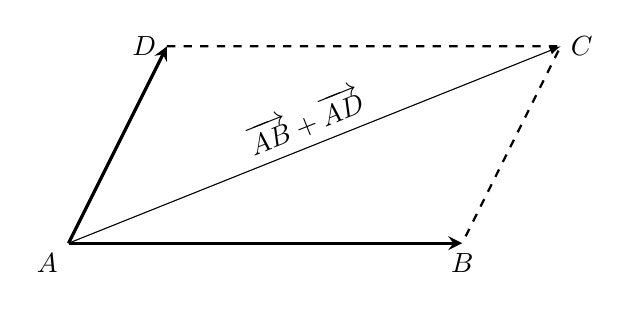
\begin{tikzpicture}[scale=2.5,>=stealth]
\draw[->,very thick](0,0)node[below left]{$A$}--++(2,0)node[below]{$B$};
\draw[->,very thick](0,0)--++(.5,1)node[left]{$D$};
\draw[dashed, thick](.5,1)--++(2,0)node[right]{$C$}--++(-.5,-1);
\draw[->,>=latex](0,0)--node[sloped, above]{$\orarrow{AB}+\orarrow{AD}$}++(2.5,1);
\end{tikzpicture}
\end{center}
\end{minipage}

物理当中力的合成是这个法则的实际模型. 物理当中力的合成是这个法则的实际模型. 物理当中力的合成是这个法则的实际模型. 物理当中力的合成是这个法则的实际模型.

\noindent
\begin{minipage}{0.6\textwidth}	
\parindent=2\ccwd\bigskip	
\indent 如图, 三角形$ABC$是边长分别为$a,b,c$的通电闭合线圈, 电流为$I$, 为逆时针方向. 若将其放置于垂直三角形所在的平面向内的匀强磁场中, 磁感应强度为$B$, 那么三条边所受到的安培力大小分别为
\begin{spacing}{1.25}
$$\begin{cases}
 F_{a}=BIa;\\
 F_{b}=BIb;\\
 F_{c}=BIc.
 \end{cases}$$
 \end{spacing} \medskip

 \noindent 闭合线圈处于平衡状态, 于是三个安培力是共点力, 作用线交于点$O$合力为0.
\end{minipage}
\begin{minipage}{0.39\textwidth}
    
\includegraphics[width=\textwidth]{1}
\end{minipage}\bigskip\bigskip




\noindent\hspace*{-20pt}
\begin{minipage}{.5\textwidth}
\begin{eqnarray*}
\lefteqn{(x^{2}+3x-3)(x^{2}+3x+5)+14}\qquad\\
&=&(t-1)(t+5)+16\\
&=&t^{2}+2t+1\\
&=&(t+1)^{2}\\
&=&(x^{2}+3x+1)^{2}
\end{eqnarray*}
\end{minipage}\hspace*{20pt}
\begin{minipage}{.49\textwidth}
视频提供了功能强大的方法帮助您证明您的观点。当您单击联机视频时,可以在想要添加的视频的嵌入代码中进行粘贴。您也可以键入一个关键字以联机搜索最适合您的文档的视频。
\end{minipage}
\medskip

%\renewcommand\arraystretch{1}
%\renewcommand {\thetable} {\thesection{}.\arabic{table}}
%
%\renewcommand {\thefigure} {\thesection{}.\arabic{figure}}

\begin{figure}[H]
\begin{center}
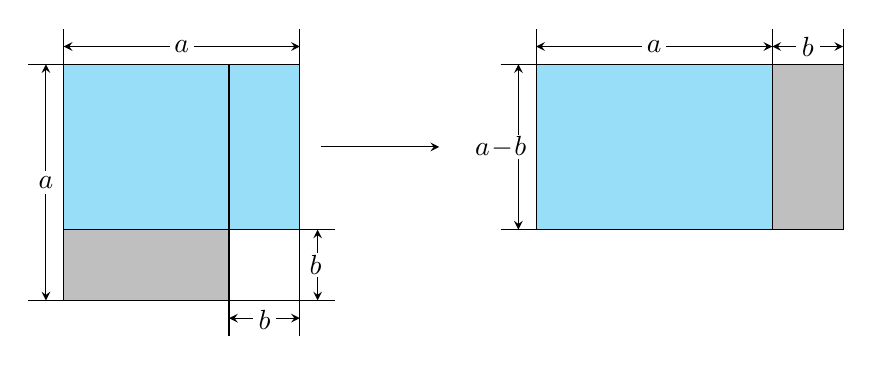
\begin{tikzpicture}[>=stealth,scale=3]
    \pgfmathsetmacro{\h}{1}
    \pgfmathsetmacro{\v}{.15}
    \pgfmathsetmacro{\a}{1}
    \pgfmathsetmacro{\b}{.3}
    \foreach \i in {{0,0},{\a+\h,0}}
    \draw[fill=cyan!40](\i)rectangle++(\a,\a-\b);
    \foreach \i/\j in {{0,0}/{\a-\b,-\b},{\a+\h+\a,0}/{\b,\a-\b}}
    \draw[fill=gray!50](\i)rectangle++(\j);
    \draw(\a,0)--node[right]{$b$}++(0,-\b) --node[below]{$b$} ++(-\b,0)--++(0,\a);
    \draw[->](\a+\b*.3,\a/2-\b/2)--++(\h*.5,0);
    \foreach \i in {-1,1}{
        \foreach \j/\len in {%
            {\a/2,\a-\b}/\a,
            {\a+\h+\a/2,\a-\b}/\a,
            {\a-\b/2,-\b-\v}/\b,
            {\a+\a+\b/2+\h,\a-\b}/\b}
            {\draw($(\j)+(\i*\len/2,0)$)--++(0,\v);
            \draw[->]($(\j)+(\i*\v/3,\v/2)$)--++({\i*(\len/2-\v/3)},0);}
        \foreach \k/\len in {%
            {-\v,\a/2-\b}/\a,
            {\a,-\b/2}/\b ,
            {\a+\h-\v,\a/2-\b/2}/(\a-\b)}
            {\draw($(\k)+(0,{\i*\len/2})$)--++(\v,0);
            \draw[->]($(\k)+(\v/2,\i*\v/3)$) --++(0,{\i*(\len/2-\v/3)});}
        }
    \foreach \i/\tex in {
        {\a/2,\a-\b+\v/2}/a,
        {\a/2+\a+\h,\a-\b+\v/2}/a,
        {-\v/2,\a/2-\b}/a,
        {\a+\h+\a+\b/2,\a-\b+\v/2}/b, {\a+\h-\v,\a/2-\b/2}/a\!-\!b}
        \draw(\i)node{$\tex$};
\end{tikzpicture}
\caption{\label{twosquare} 两个矩形.}
\end{center}
\end{figure}


\section{一个修正排版范例}
\subsection{初始排版}
\begin{thm}\label{thm}
常数项级数$\sum\limits_{n=1}^{\infty}{w_n}$收敛等价于存在分解式$w_n={u_n}{v_n}$ 使得数列$\{u_n\}$单调且$\displaystyle\lim_{n\to{\infty}}u_n=0$, 级数$\sum\limits_{n=1}^{\infty}{v_n}$的部分和数列有界即对$\forall k\in\mathbb{ N^{*}}$, 存在正整数$ M$, 恒有$\vert\sum\limits_{n=1}^{k}{v_n}\vert< M$.
\end{thm}
\begin{proof}
充分性见复旦大学编数学分析下册.

下证必要性\\
由常数项级数$\sum\limits_{n=1}^{\infty}{w_n}$收敛知
$\forall\varepsilon>0$, $\exists  N\in\mathbb{ N^{*}}$, 当$k\geq N$ 时,有${\vert{\sum\limits_{n=1}^{\infty}{w_n}}\vert}<\varepsilon$\\
取$\varepsilon=1$; $\exists  N_1\in\mathbb{ N^{*}}$, 当$k\geq N_1$ 时,有${\vert{\sum\limits_{n=k}^{\infty}{w_n}}\vert}<1$\\
$\varepsilon=\frac{1}{2^3}$; $\exists  N_2\in\mathbb{ N^{*}}>N_{1}$, 当$k\geq N_2$ 时,有${\vert{\sum\limits_{n=k}^{\infty}{w_n}}\vert}<\frac{1}{2^3}$\\
$$\vdots$$\\
$\varepsilon=\frac{1}{i^3}$; $\exists  N_i\in\mathbb{ N^{*}}>N_{i-1}$, 当$k\geq N_i$ 时,有${\vert{\sum\limits_{n=k}^{\infty}{w_n}}\vert}<\frac{1}{i^3}$\\
$$\vdots$$\\
令
$$
{u_n}=\bigg\{\!\!\!
\begin{array}{ll}
1,&n=1,2,\idots,N_1;\\[-15pt]
\frac{1}{i},&N_i<n\leq N_{i+1}, k=1,2,3,\dots.
\end{array}
$$
故有数列$\{u_n\}$单调且$\displaystyle \lim_{n\to{\infty}}u_n=0$\\
令$v_n=\frac{w_n}{u_n}$,则\\
(a)当$k\leq N_1$, 由$u_n=1$知$v_n=w_n$, 所以有\\
$\vert{\sum\limits_{n=1}^{k}{v_n}}\vert=\vert{\sum\limits_{n=1}^{k}{w_n}}\vert\leq{\sum\limits_{n=1}^{k}{\vert{w_n}\vert}}
\leq{\sum\limits_{n=1}^{N_1}{\vert{w_n}\vert}}$\\
记${\sum\limits_{n=1}^{N_1}{\vert{w_n}\vert}}$为$ M_1$, 则有 ${\vert{\sum\limits_{n=1}^{k}{v_n}}\vert}\leq M_1$\\
(b)当$k>N_1$, 则一定存在$i$使得$N_i<k\leq N_{i+1}$, 则有\\
\begin{eqnarray*}
\lefteqn{\vert\sum_{n=1}^{k}v_n\vert}\\
&=&\vert\sum_{n=1}^{k}\frac{w_n}{u_n}\vert\\
&=&\vert\sum_{n=1}^{N_1}{w_n}+\sum_{N_1+1}^{N_2}w_n +\dots+i\sum_{N_i+1}^{k}w_n\vert\\
&\le&\vert\sum_{n=1}^{N_1}w_n\vert +\vert\sum_{N_1+1}^{N_2}w_n\vert+\dots +i\vert\sum_{N_i+1}^{k}w_n\vert\\
&=&\vert\sum_{n=1}^{N_1}w_n\vert+\vert\bigg(\sum_{N_1+1}^{+\infty}w_n -\sum_{N_2+1}^{+\infty}w_n\bigg)\vert +\dots+i\vert\sum_{N_i+1}^{+\infty}w_n -\sum_{k+1}^{+\infty}w_n\vert\\
&\le&\vert\sum_{n=1}^{N_1}w_n\vert+ \bigg(\vert\sum_{N_1+1}^{+\infty}w_n\vert+\vert\sum_{N_2+1}^{+\infty}w_n \vert\bigg) +\dots+i\bigg(\vert\sum_{N_i+1}^{+\infty}w_n\vert +\vert\sum_{k+1}^{+\infty}w_n\vert\bigg)\\
&<& M_1+\bigg(1+\frac1{2^3}\bigg) +\dots+i\bigg(\frac1{i^3}+\frac1{i^3}\bigg)\\
&<& M_1+(1+1)+2\bigg(\frac1{2^3}+\frac1{2^3}\bigg) +\dots+i\bigg(\frac1{i^3}+\frac1{i^3}\bigg)\\
&=& M_1+2\bigg(1+\frac1{2^2}+\dots+\frac1{i^2}\bigg)\\
&<& M_1+2\sum\frac1{i^2}\\
&=& M_1+2\times\frac\pi6\\
&=& M_1+\frac\pi3
\end{eqnarray*}
\end{proof}
\subsection{修正排版}
\begin{thm}\label{thm}
常数项级数$\sum_{n=1}^{\infty}{w_n}$收敛等价于存在分解式$w_n={u_n}{v_n}$使得数列$\{u_n\}$单调且$\lim_{n\to{\infty}}u_n=0$, 级数$\sum_{n=1}^{\infty}{v_n}$的部分和数列有界即对\textcolor{red}{任意}$k\in\mathbb{N}^*$, 存在正整数$M$, 使得$\vert\sum_{n=1}^{k}{v_n}\vert<M$.
\end{thm}
\begin{proof}
    充分性见复旦大学编数学分析下册. 下证必要性. 由常数项级数$\sum_{n=1}^{\infty}{w_n}$收敛知对任意$\varepsilon>0$, 存在$N\in\mathbb{N}^*$, 使得当$k\ge N$ 时, 有$\vert\sum_{n=1}^{\infty}w_n\vert<\varepsilon$. 取$\varepsilon=k^{-3}$, 令$N_k$为相应的正整数$N$使得, $n>N$时有$\vert\sum_{n>N}^\infty w_n\vert<\varepsilon$. 令
    $$u_n=\begin{cases}
        1,&1\le n\le N_1;\\
        \dfrac1i,&N_i<n\le N_{i+1}, i\ge1.
    \end{cases}$$
    故数列$\{u_n\}$单调且$\lim_{n\to{\infty}}u_n=0$. 令$v_n=\frac{w_n}{u_n}$, 则

    (a) 当$k\le N_1$, 由$u_n=1$知$v_n=w_n$, 所以有$$\vert\sum_{n=1}^{k}{v_n}\vert=\vert\sum_{n=1}^{k}{w_n}\vert \le\sum\limits_{n=1}^{k}{\vert{w_n}\vert}\le\sum_{n=1}^{N_1}\vert w_n\vert.$$ 记$\sum_{n=1}^{N_1}\vert w_n\vert$为$M_1$, 则有 $\vert\sum_{n=1}^kv_n\vert\le M_1$.

    (b) 当$k>N_1$, 则一定存在$i$使得$N_i<k\le N_{i+1}$, 则有\setcolsep
    \begin{eqnarray*}
    \Big\vert\sum_{n=1}^{k}v_n\Big\vert
        &=&\Big\vert\sum_{n=1}^{k}\frac{w_n}{u_n}\Big\vert\\
        &=&\Big\vert\sum_{n=1}^{N_1}{w_n}+\sum_{N_1+1}^{N_2}w_n +\cdots+i\sum_{N_i+1}^{k}w_n\Big\vert\\
        &\le&\Big\vert\sum_{n=1}^{N_1}w_n\Big\vert +\Big\vert\sum_{N_1+1}^{N_2}w_n\Big\vert+\cdots +i\Big\vert\sum_{N_i+1}^{k}w_n\Big\vert\\
        &=&\Big\vert\sum_{n=1}^{N_1}w_n\Big\vert+\Big\vert\bigg(\sum_{N_1+1}^{+\infty}w_n -\sum_{N_2+1}^{+\infty}w_n\bigg)\Big\vert +\cdots+i\Big\vert\sum_{N_i+1}^{+\infty}w_n -\sum_{k+1}^{+\infty}w_n\Big\vert\\
        &\le&\Big\vert\sum_{n=1}^{N_1}w_n\Big\vert+ \bigg(\Big\vert\sum_{N_1+1}^{+\infty}w_n\Big\vert+\Big\vert\sum_{N_2+1}^{+\infty}w_n \Big\vert\bigg) +\cdots+i\bigg(\Big\vert\sum_{N_i+1}^{+\infty}w_n\Big\vert +\Big\vert\sum_{k+1}^{+\infty}w_n\Big\vert\bigg)\\
        &<& M_1+\bigg(1+\frac1{2^3}\bigg) +\cdots+i\bigg(\frac1{i^3}+\frac1{i^3}\bigg)\\
        &<& M_1+(1+1)+2\bigg(\frac1{2^3}+\frac1{2^3}\bigg) +\cdots+i\bigg(\frac1{i^3}+\frac1{i^3}\bigg)\\
        &=& M_1+2\bigg(1+\frac1{2^2}+\cdots+\frac1{i^2}\bigg)\\
    &<& M_1+2\sum\frac1{i^2}=M_1+2\times\frac\pi6
    = M_1+\frac\pi3.
    \end{eqnarray*}
    证毕
\end{proof}


\subsection{下面例子需要大家动手修改}
证明与定理2.3类似,但是有一个问题我们需要注意.数列收敛则一定有数列有界,但是函数列一致收敛不能推出函数列一致有界,因此我们需要对函数列$\{u_n(x)\}$做一些修改.
\begin{thm}\label{thm}
函数项级数$\sum_{n=1}^{\infty}{w_n(x)}$在区间$D=[a,b]$上一致收敛等价于存在分解式$w_n(x)={u_n(x)}{v_n(x)}$ 使得函数列$\{u_n(x)\}$ 对每一个固定的$x\in D$关于n单调且在区间$D$上$\{u_n(x)\}\rightrightarrows0$, 函数项级数$\sum_{n=1}^{\infty}{v_n(x)}$ 的部分和序列一致有界即对$\forall k\in\mathbb{N}^{*}$, 存在正整数$ M$, 对$\forall x\in D$恒有$\vert\sum_{n=1}^{k}{v_n(x)}\vert< M$.
\end{thm}

\begin{proof}
充分性见复旦大学编数学分析下册

下证必要性\\
由函数项级数$\sum\limits_{n=1}^{\infty}{w_n(x)}$在区间$[a,b]$上一致收敛知
$\forall\varepsilon>0$, $\exists  N\in\mathbb{ N^{*}}$, 当$k\geq N$ 时,有${\vert{\sum\limits_{n=1}^{\infty}{w_n(x)}}\vert}<\varepsilon$ 对 $\forall x\in D$均成立\\
取$\varepsilon=1$; $\exists  N_1\in\mathbb{ N^{*}}$, 当$k\geq N_1$ 时,有${\vert{\sum\limits_{n=k}^{\infty}{w_n(x)}}\vert}<1$\qquad$\forall x\in D$\\
$\varepsilon=\frac{1}{2^3}$; $\exists  N_2\in\mathbb{ N^{*}}>N_{1}$, 当$k\geq N_2$ 时,有${\vert{\sum\limits_{n=k}^{\infty}{w_n(x)}}\vert}<\frac{1}{2^3}$\qquad$\forall x\in D$\\
$$\vdots$$\\
$\varepsilon=\frac{1}{i^3}$; $\exists  N_i\in\mathbb{ N^{*}}>N_{i-1}$, 当$k\geq N_i$ 时,有${\vert{\sum\limits_{n=k}^{\infty}{w_n(x)}}\vert}<\frac{1}{i^3}$\qquad$\forall x\in D$\\
$$\vdots$$\\
令$E={x\mid{\vert{\sum\limits_{n=1}^{N_1}{w_n(x)}}\vert<1},x\in D}$\\
$$
{s(x)}=\bigg\{\!\!\!
\begin{array}{ll}
1,&x\in E;\\[-15pt]
\vert{\sum\limits_{n=1}^{N_1}{w_n(x)}}\vert,&x\in{D\bigcap E^c}.
\end{array}
$$
令
$$
{u_n(x)}=\bigg\{\!\!\!
\begin{array}{ll}
s(x),&n=1,2,\ldots,N_1;\\[-15pt]
\frac{1}{i},&N_i<n\leq N_{i+1}, k=1,2,3,\dots.
\end{array}
$$
故(1)当$x\in E$,$\{u_n(x)\}=\{1,1,\frac{1}{2},\cdots\}$\\
(2)当$x\in{D\bigcap E^c}$时,则$\vert{\sum\limits_{n=1}^{N_1}{w_n(x)}}\vert\geq 1$, 故$\{u_n(x)\}=\{\vert{\sum\limits_{n=1}^{N_1}{w_n(x)}}\vert,1,\frac{1}{2},\cdots\}$\\
所以函数列$\{u_n(x)\}$ 对每一个固定的$x\in D$关于n单调且在区间$D$上$\{u_n(x)\}\rightrightarrows0$\\
令$v_n(x)=\frac{w_n(x)}{u_n(x)}$,则\\
(a)当$k\leq N_1$有
$\vert\sum_{n=1}^kv_n(x)\vert=\vert\sum_{n=1}^k\frac{w_n(x)}{u_n(x)}\vert=
\vert\sum_{n=1}^k\frac{w_n(x)}{s(x)}\vert
\le\frac{\sum_{n=1}^k\vert w_n(x)\vert}{s(x)}
\le\frac{\sum_{n=1}^{N_1}\vert w_n(x)\vert}{s(x)}\le 1$.

(b)当$k>N_1$, 则一定存在$i$使得$N_i<k\leq N_{i+1}$, 则有\\
\begin{eqnarray*}
\lefteqn{\vert\sum_{n=1}^{k}v_n(x)\vert}\\
&=&\vert\sum_{n=1}^k\frac{w_n(x)}{u_n(x)}\vert\\
&=&\vert\sum_{n=1}^{N_1}\frac{w_n(x)}{u_n(x)} +\sum_{N_1+1}^{N_2}w_n(x)+\dots+i\sum_{N_i+1}^kw_n(x)\vert\\
&\le&1+\vert\sum_{N_1+1}^{N_2}w_n(x)\vert+\dots +i\vert\sum_{N_i+1}^kw_n(x)\vert\\
&=&1+\vert\bigg(\sum_{N_1+1}^{+\infty}w_n(x) -\sum_{N_2+1}^{+\infty}w_n(x)\bigg)\vert +\dots +i\vert\sum_{N_i+1}^{+\infty}w_n(x)-\sum_{k+1}^{+\infty}w_n(x)\vert\\
&\le&1+\bigg(\vert\sum_{N_1+1}^{+\infty}w_n(x)\vert+ \vert\sum_{N_2+1}^{+\infty}w_n(x)\vert\bigg)+\dots +i\bigg(\vert\sum_{N_i+1}^{+\infty}w_n(x)\vert +\vert\sum_{k+1}^{+\infty}w_n(x)\vert\bigg)\\
&<&1+\bigg(1+\frac1{2^3}\bigg)+\dots+i\bigg(\frac1{i^3}+\frac1{i^3}\big)\\
&<&1+(1+1)+2\bigg(\frac1{2^3}+\frac1{2^3}\bigg)+\dots +i\bigg(\frac1{i^3}+\frac1{i^3}\bigg)\\
&=&1+2\bigg(1+\frac{1}{2^2}+\dots+\frac{1}{i^2}\bigg)\\
&<&1+2\sum\frac{1}{i^2}\\
&=&1+2\times\frac\pi6\\
&=&1+\frac\pi3
\end{eqnarray*}
\end{proof}


\begin{lemma}\label{lem8}
若$u=(v_1, v_2)$是$F_T(v)$的一个奇点, 则$y_0=\dfrac{u}{v_i}$或$y_0=-\dfrac{u}{v_i}$是系统
\eqref{eqabcd3} 的奇点. %这里直接截取了原论文,因此没有编号
\end{lemma}

\begin{proof}
由于$u=(v_1, v_2)$是$F_T(v)$的一个奇点, 则$F_T(u)=0 \rightarrow h(u)-uQ(u)=0$, 即$h_i(u)-v_i Q(u)=0, i=1, 2$.
\noindent 当$y_0=\dfrac{u}{v_i}$时,
    $$h(y_0)-y_0 h_i(y_0)=\dfrac{uQ(u)}{v_i}-\dfrac{u h_i(u)}{v_i^2}=0;$$
当$y_0=-\dfrac{u}{v_i}$时,
    $$h(y_0)+y_0 h_i(y_0)=-\dfrac{uQ(u)}{v_i}+\dfrac{u h_i(u)}{v_i^2}=0.$$
得证.
\end{proof}

\begin{spacing}{1}\zihao{-4}
$$\begin{cases}
\dfrac{\dev y_1}{\dev t}=-a_2(y_1-\delta_1)(y_1-\delta_2);\\[5pt]
\dfrac{\dev y_2}{\dev t}=0.
\end{cases}$$
\end{spacing}\bigskip




    \newpage
%正文结束

%参考文献
\begin{thebibliography}{99}
\addcontentsline{toc}{section}{\protect 参考文献}
\setlength{\itemsep}{-0.75ex}
% 请把文献条目填写在下面, 例如
\bibitem{zhs}张三. 钢铁侠[J]. 数学实践, 2020, \textbf{10}2: 1-10.
\end{thebibliography}
\newpage
\section*{\centerline{致 \quad 谢}}
\addcontentsline{toc}{section}{\protect 致谢}
感谢!
\newpage
\section*{附录}
\addcontentsline{toc}{section}{\protect 附录}
此节可添加调查问卷、访谈记录等
\newpage
\nocite{*}
%\setlength{\bibitemsep}{-0.75ex}
%\titleformat{command}[shape]{format}{label}{sep}{before}[after]
\renewcommand{\bibfont}{\zihao{-4}}
\printbibliography[heading=bibintoc,title=\zihao{4}参考文献]
%\nocite{*}
%\bibliography{reference}
\end{document}